\documentclass[11pt,letterpaper]{article}
\usepackage{style}

%% ------- INICIA DOCUMENTO ------
\begin{document}
\begin{titlepage}
\begin{center}
\begin{LARGE}
INSTITUTO POLITÉCNICO NACIONAL\\
\vspace*{0.15in}
ESCUELA SUPERIOR DE CÓMPUTO\\
\end{LARGE}
\vspace*{1.0in}
\begin{Large}
%% NOMBRE DE LA PRÁCTICA O EXAMEN
\textbf{TÉCNICAS DE CRUZA 1} \\  
\end{Large}
\vspace*{0.2in}
\begin{large}
\textit{Práctica 6}\\
\end{large}
\vspace*{1.0in}
\begin{large}
%% INTEGRANTES	
Dominguez de la Rosa Bryan\\
\vspace*{2.0in}
GRUPO 3CM5\\
\vspace*{0.2in}
Profesor: Morales Güitron Sandra Luz\\
\vspace*{1.5in}
\today
\vspace*{0.3in}
\end{large}
\rule{150mm}{0.1mm}\\

\end{center}
\end{titlepage}

%% --------- COMIENZA EL DESARROLLO DEL DOCUMENTO --------

\section*{Introducción}
La idea básica del método de selección por torneo es escoger individuos con base en comparaciones directas entre ellos.\\

Hay 2 versiones de la seleccion mediante torneo:
\begin{itemize}
	\item Determinística.
	\item Probabilística.
\end{itemize}

\noindent
En esta práctica implementamos la versión probabilística, la cual realiza los siguientes pasos:
\begin{enumerate}
	\item Barajar los individuos de la población.
	\item Escoger un número p de individuos (normalmente 2).
	\item Compararlos con base en su aptitus.
	\item Generar un \textit{flip}.
	\item Elegir al individuo más apto si \textit{flip} resulta verdadero, en caso contrario se elige al individuo menos apto.
\end{enumerate}


\section*{Contenido}
Para la implementación del algoritmo de selección por torneo, implementé 4 arreglos de bits para controlar las distintas etapas que se realizan en el algoritmo:
\begin{itemize}
	\item Población inicial.
	\item Población de individuos seleccionados mediante el algoritmo de selección por torneo.
	\item Población después de cruza.
	\item Población después de mutación.
\end{itemize}


En la primer etapa, se llena aleatoriamente el arreglo de población inicial con series de 5 bits. Después, para implementar la selección por torneo, se barajean los individuos de la población, con el fin de generar parejas para el enfrentamiento. Al darse el primer enfrentamiento, se seleccionan 16 individuos ganadores, por lo que es necesario barajear de nuevo la población y volver a realizar el algoritmo, para de este modo completar los 32 individuos que tenía nuestra población original.\\

Una vez teniendo la población de selección de padres, se realiza una cruza de individuos de la siguiente manera:

\begin{enumerate}
	\item Se utilizan 2 individuos de la población de padres.
	\item Se define un punto de cruza estático para todas las generaciones.
	\item Se cruzan los individuos.
	\item Se retorna el individuo resultante.
\end{enumerate}

\begin{figure}[H]
	\centering
	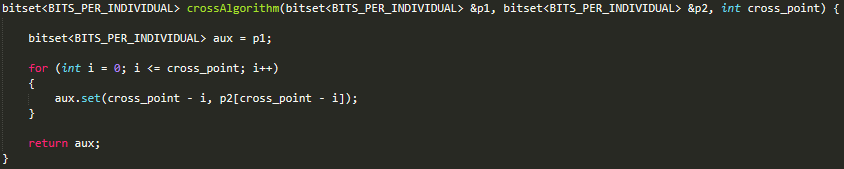
\includegraphics[scale = .8]{images/cruza}
	\caption{Algoritmo de cruza de individuos}
\end{figure}

Al obtener la población de individuos después de la cruza se necesita realizar una mutación. En este caso se generó una mutación del 10\% de la población. Nuestra población total es de 32 elementos, entonces la cantidad de individuos a redondear es 3.2, redondeado como 3.\\

La mutación se realiza de la siguiente forma:
\begin{enumerate}
	\item El algoritmo se realizará 3 veces.
	\item La mutación buscará mejorar al individuo, por lo tanto, se buscará cambiar un bit 0 por un bit 1.
	\item Debido a que se requiere buscar un 0 en el individuo a mutar, y es posible que el individuo no tenga bits 0, se define un número máximo de iteraciones para evitar que el programa se cicle.
	\item Cuando se encuentre un bit 0, se cambia por un bit 1.
\end{enumerate}

\begin{figure}[H]
	\centering
	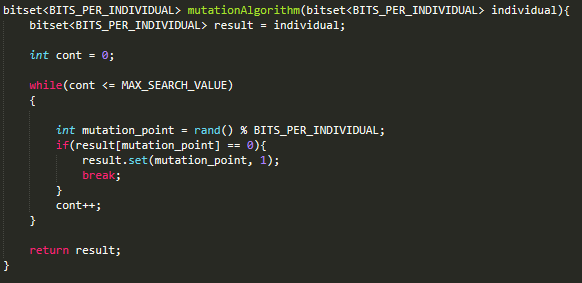
\includegraphics[scale = 1]{images/mutacion}
	\caption{Algoritmo de mutación de individuos}
\end{figure}

Una vez que se tenga la población mutada, se establece ésta como población inicial, para realizar el algoritmo de ruleta en la siguiente generación.\\

Al obtener la población final de una generación, se obtiene la aptitud del individuo de menor valor, la aptitud del individuo de mayor valor y el promedio de aptitud de cada generación.\\

A continuación se muestran 2 ejemplos con 10, 30, 50 y 100 generaciones, en los que la línea azul representa la aptitud del mejor individuo de cada generación, la línea roja representa la aptitud del peor individuo de cada generación y la línea blanca representa el promdedio de aptitud de cada generación.
\begin{figure}[H]
	\centering
	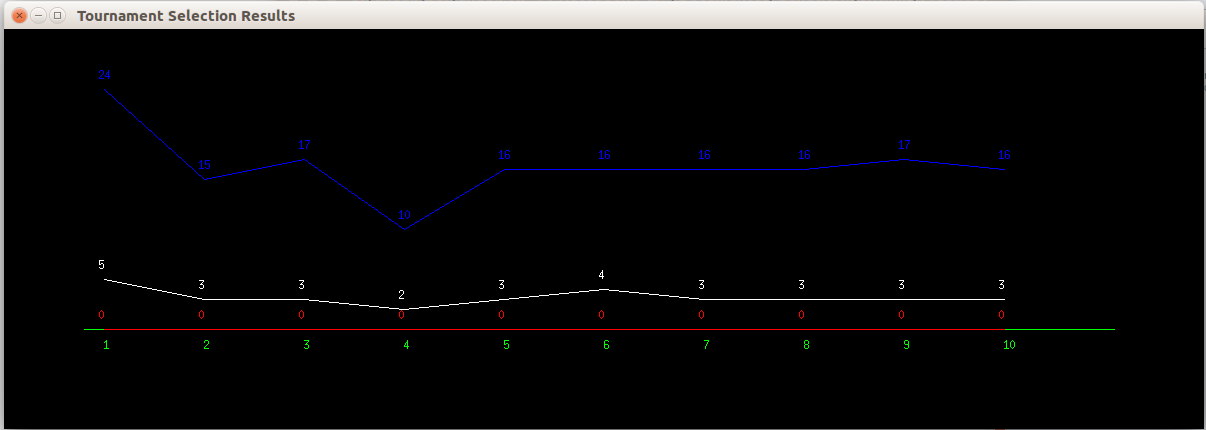
\includegraphics[scale = 0.4]{images/10gen1}
	\caption{Resultado 1 con 10 generaciones}
\end{figure}

\begin{figure}[H]
	\centering
	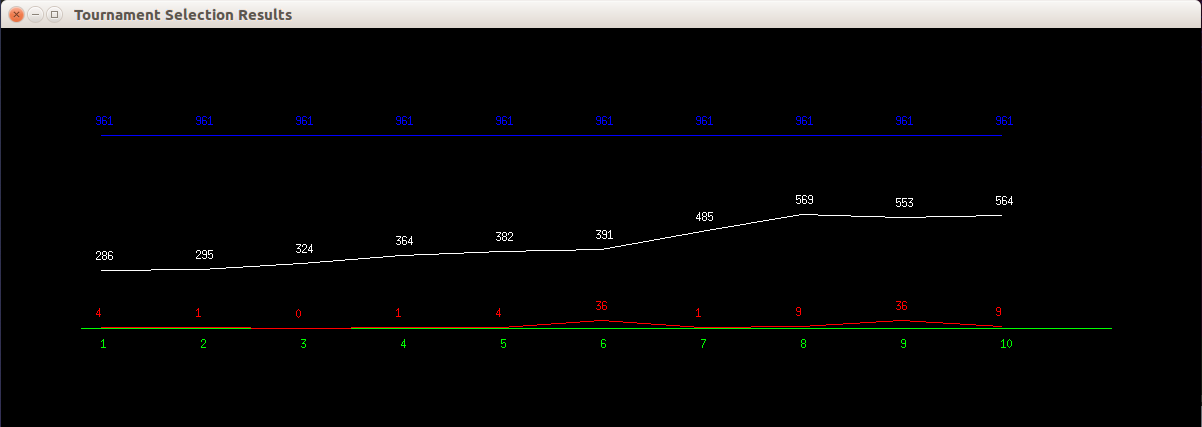
\includegraphics[scale = 0.4]{images/10gen2}
	\caption{Resultado 2 con 10 generaciones}
\end{figure}

\begin{figure}[H]
	\centering
	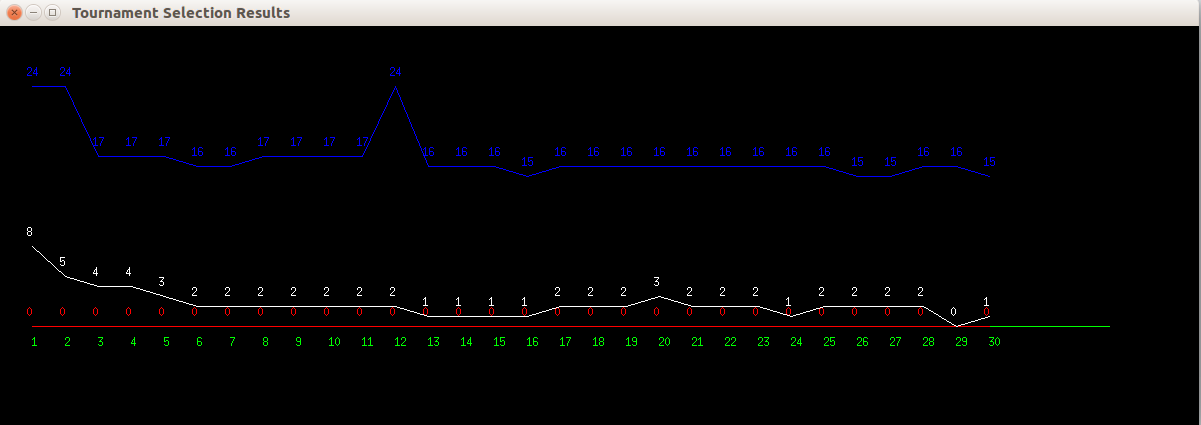
\includegraphics[scale = 0.4]{images/30gen1}
	\caption{Resultado 1 con 30 generaciones}
\end{figure}

\begin{figure}[H]
	\centering
	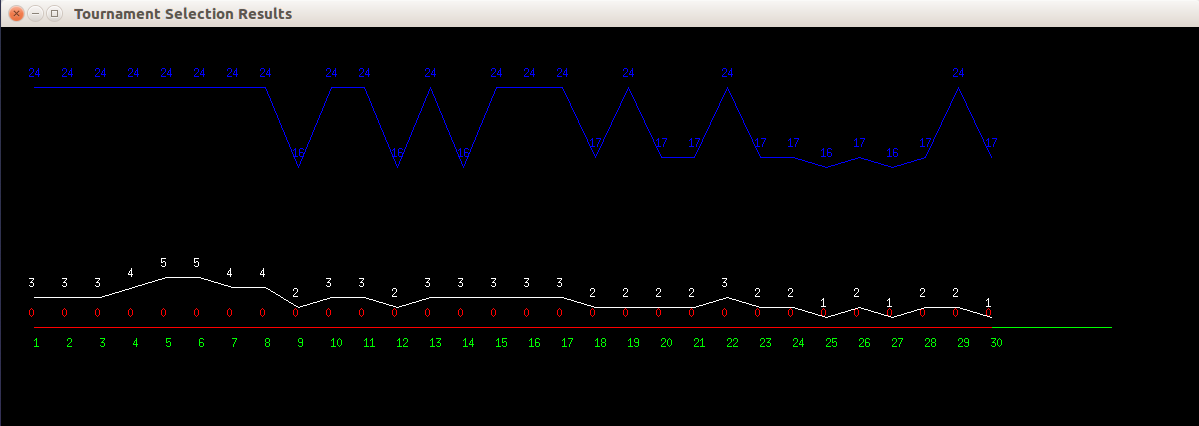
\includegraphics[scale = 0.4]{images/30gen2}
	\caption{Resultado 2 con 30 generaciones}
\end{figure}

\begin{figure}[H]
	\centering
	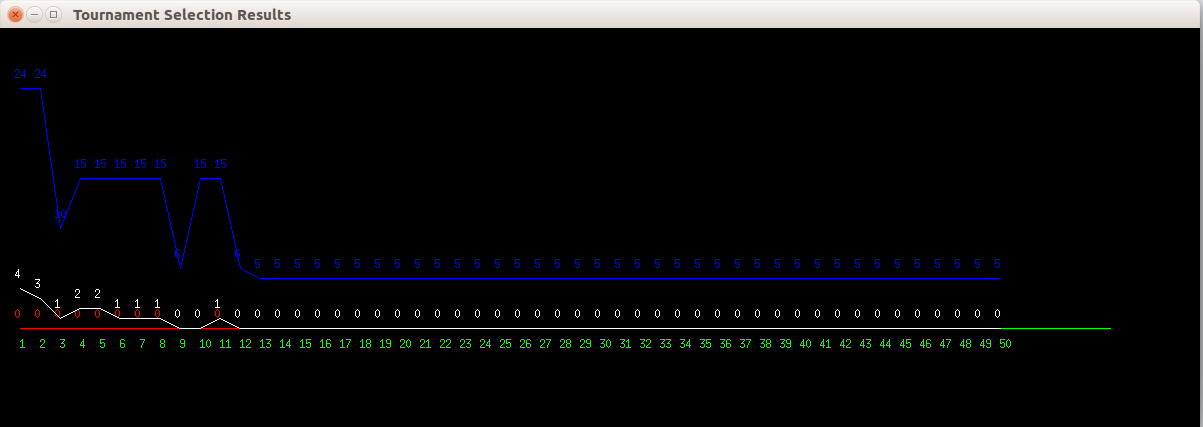
\includegraphics[scale = 0.4]{images/50gen1}
	\caption{Resultado 1 con 50 generaciones}
\end{figure}

\begin{figure}[H]
	\centering
	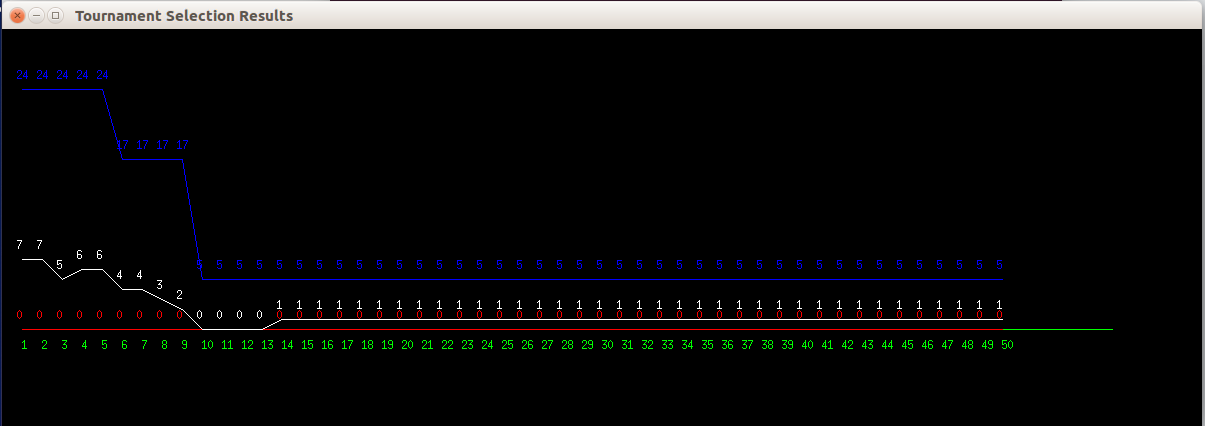
\includegraphics[scale = 0.4]{images/50gen2}
	\caption{Resultado 2 con 50 generaciones}
\end{figure}

\begin{figure}[H]
	\centering
	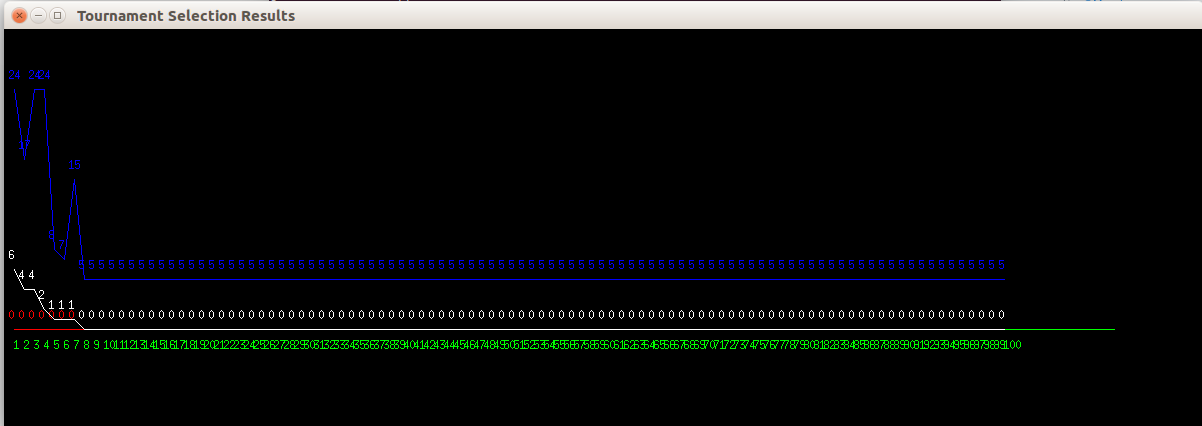
\includegraphics[scale = 0.4]{images/100gen1}
	\caption{Resultado 1 con 100 generaciones}
\end{figure}

\begin{figure}[H]
	\centering
	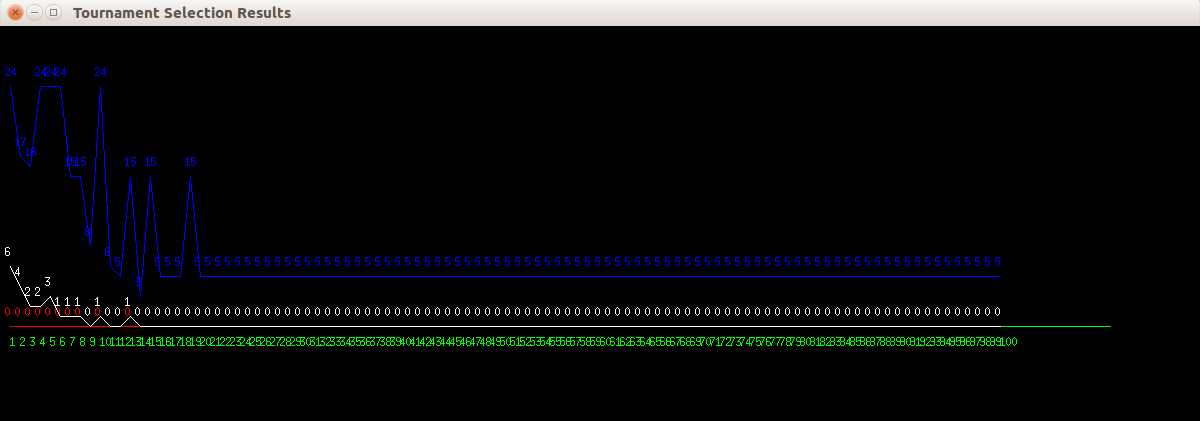
\includegraphics[scale = 0.4]{images/100gen2}
	\caption{Resultado 2 con 100 generaciones}
\end{figure}


\section*{Conclusión}

La selección probabilística implica que los individuos que resultan ser seleccionados pueden no ser los más aptos, a diferencia de la selección determinista, que siempre nos entregará como resultado un individuo más apto que su rival.\\

En la naturaleza, existen muchos factores que determinan que un individuo pueda resultar ganador en un enfrentamiento, y no siempre el más apto resulta ganador, por lo que el algoritmo probabilístico resulta ser una simulación más cercana a la realidad.

\end{document}


